\documentclass{article}

\usepackage{graphicx} 
\usepackage{subfigure}
\usepackage{paralist}

\usepackage{hyperref}

\usepackage{url}
\usepackage{booktabs}

\usepackage[usenames,dvipsnames]{xcolor}
\usepackage{tikz}
\usetikzlibrary{positioning, calc}

\usepackage[draft,nomargin,footnote]{fixme}

\graphicspath{{figs/}}

\usepackage{xspace}
\newcommand{\eg}{\textit{e.g.}\xspace}
\newcommand{\etal}{\textit{et al.}\xspace}
\newcommand{\ie}{\textit{i.e.}\xspace}
\newcommand{\etc}{\textit{etc.}\xspace}
\newcommand{\vs}{\textit{vs.}\xspace}

\title{Learning by Teaching a Robot: the Case of Handwriting}

\author{S\'everin Lemaignan, Alexis Jacq, Fernando Garcia, Ana Paiva, Pierre
Dillenbourg \\ CHILI Lab, \'Ecole Polytechnique F\'ed\'erale de Lausanne}


\begin{document}
\maketitle

\begin{abstract}
    TDB
\end{abstract}


%%%%%%%%%%%%%%%%%%%%%%%%%%%%%%%%%%%%%%%%%%%%%%%%%%%%%%%%%%%%%%%%%%%%%%%%%%%%%%%%%%%
%%%%%%%%%%%%%%%%%%%%%%%%%%%%%%%%%%%%%%%%%%%%%%%%%%%%%%%%%%%%%%%%%%%%%%%%%%%%%%%%%%%
%%%%%%%%%%%%%%%%%%%%%%%%%%%%%%%%%%%%%%%%%%%%%%%%%%%%%%%%%%%%%%%%%%%%%%%%%%%%%%%%%%%
\section{A different paradigm for educative robots}

Henry is five and an half, and has been diagnosed with visuo-constructive
deficits. He is under the care of an occupational therapist, and tries to improve
his inability to draw letters in a consistent manner. Diego is six and struggles
at school with his poor handwriting and even poorer self-confidence.

While Henry is lively and always quick at shifting his attention from one
activity to another, Diego is shy and poised. Two very different children,
facing however the same difficulty to write in a legible manner.


\begin{figure}
    \centering
    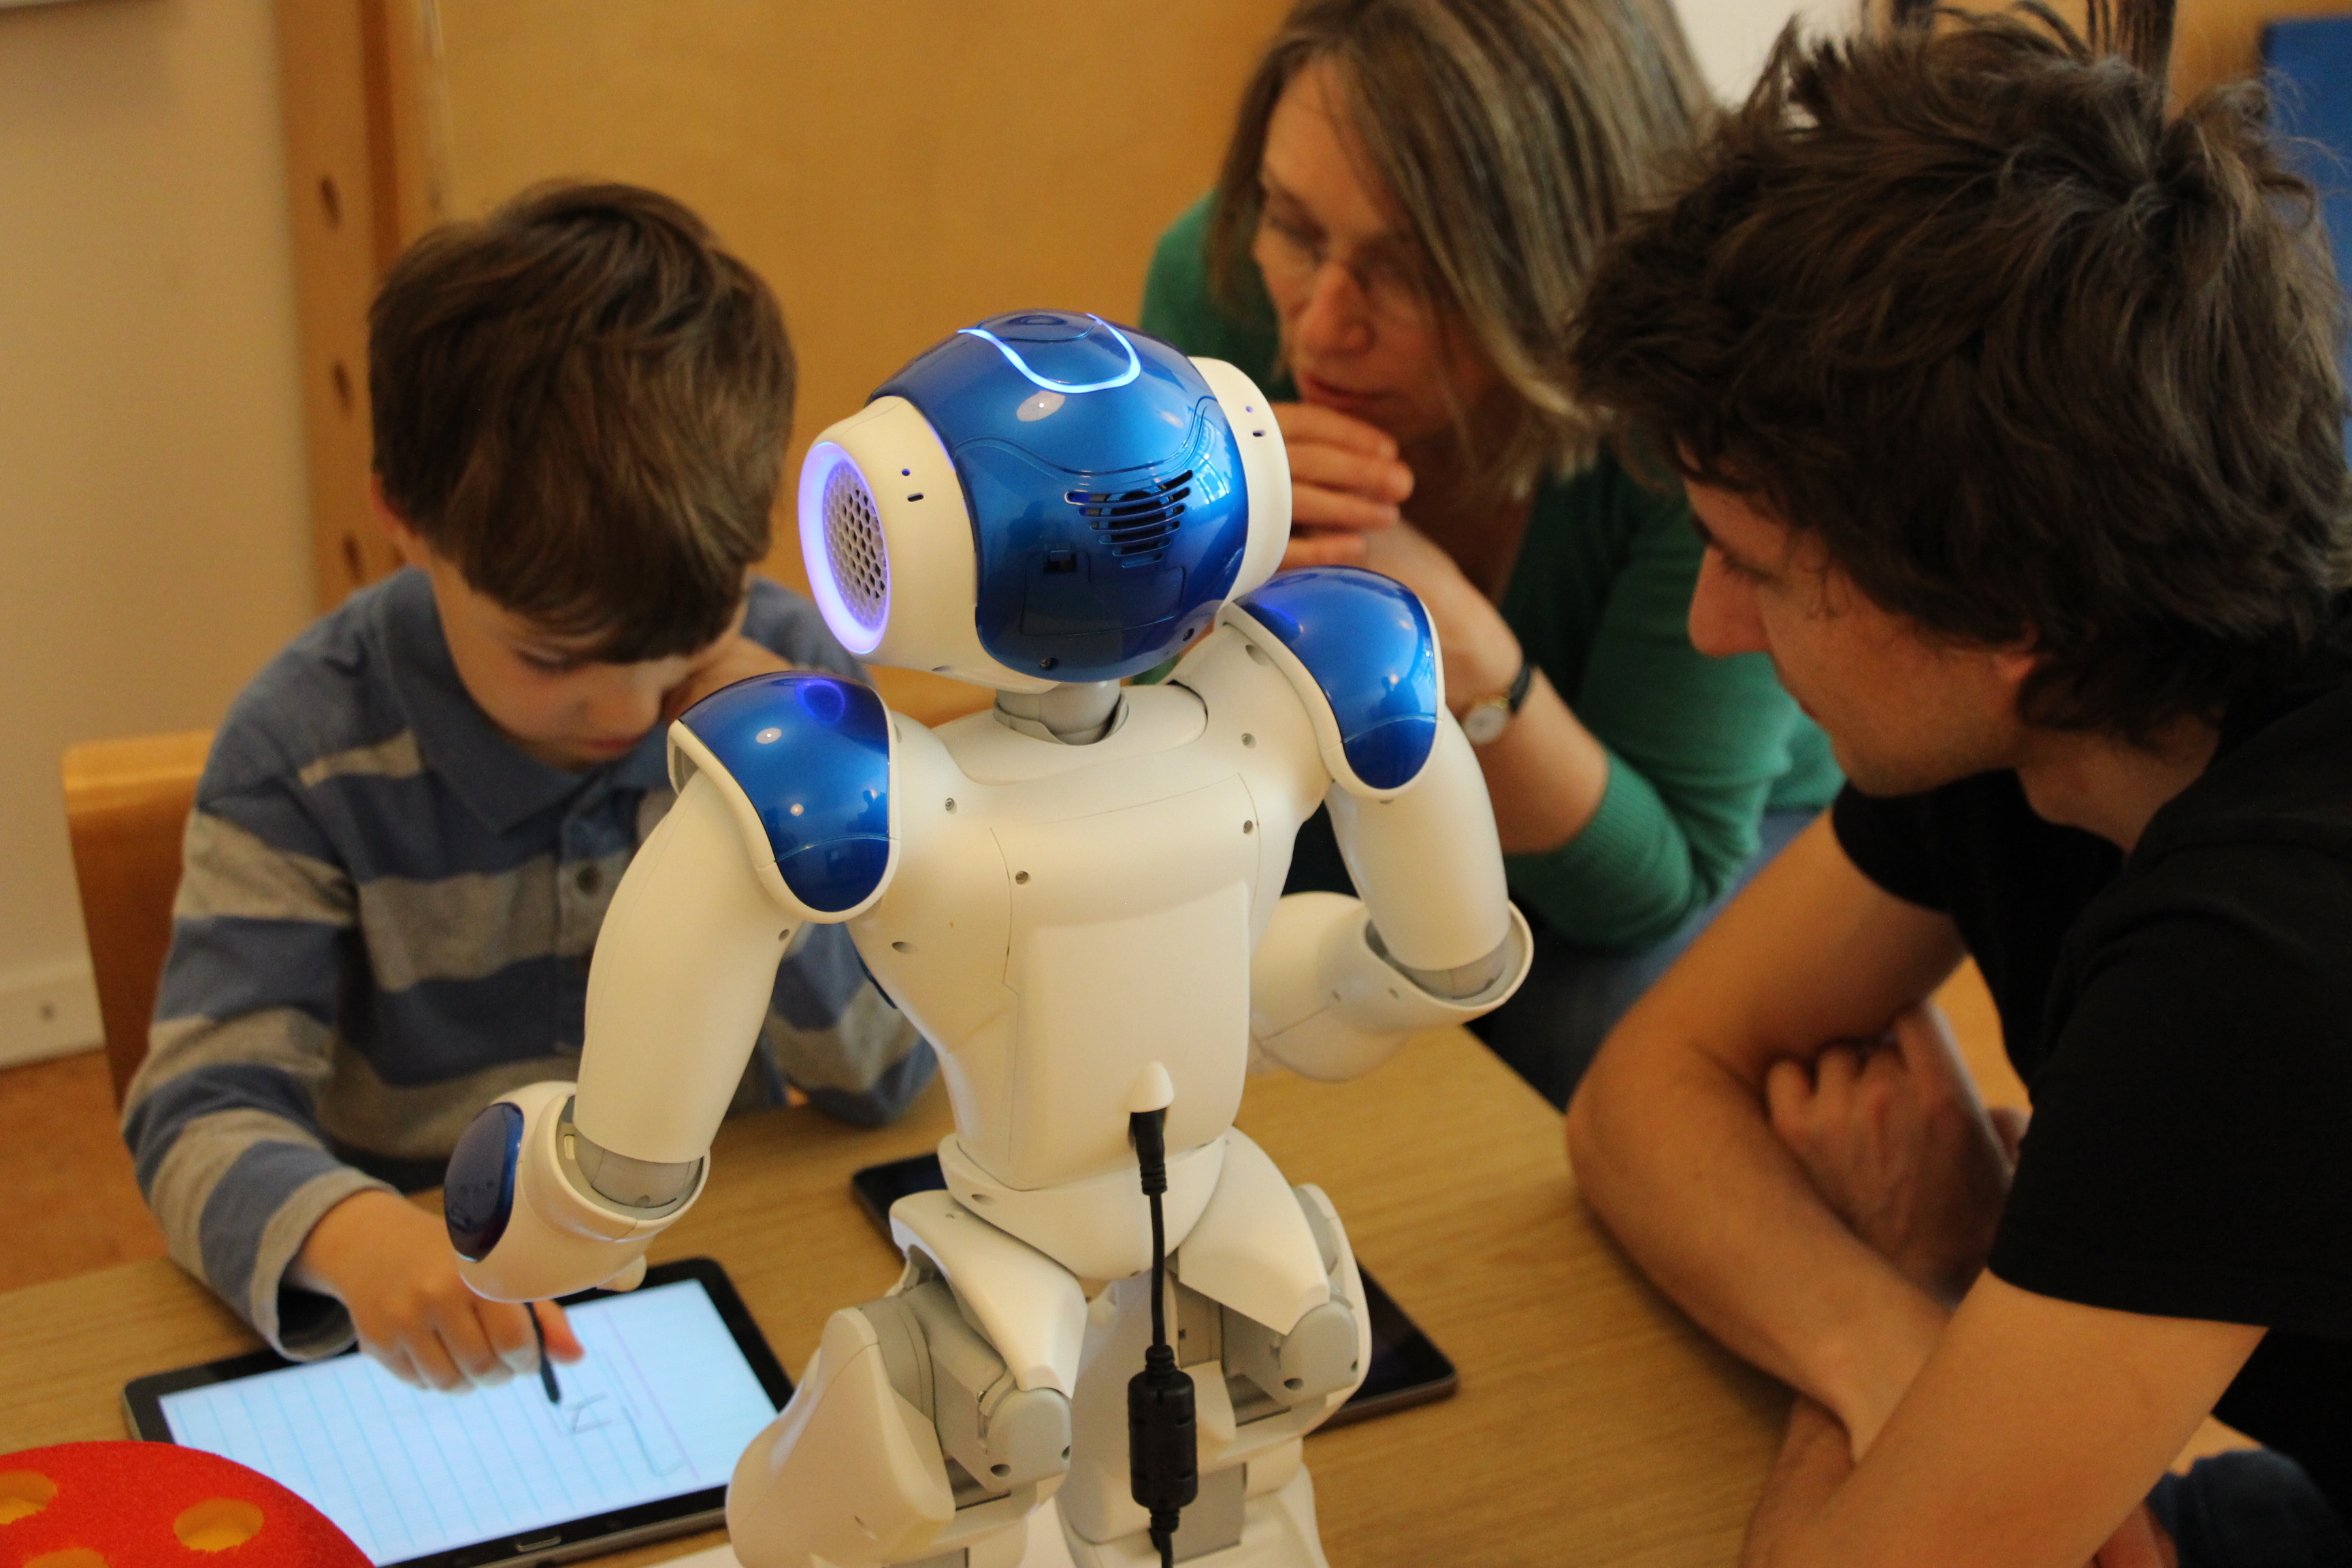
\includegraphics[width=0.9\linewidth]{henry}
    \caption{Henry teaching Nao how to write numbers, with the help of an
    occupational therapist.}
    \label{fig:henry}
\end{figure}

Remediations for handwriting difficulties

\subsection{Learning by Teaching}

The \emph{learning by teaching} paradigm, which engages the target student in
the act of teaching another, has been shown to produce motivational,
meta-cognitive, and educational benefits in a range of disciplines~\cite{Rohrbeck2003}. 
To our best knowledge, the application of the paradigm to
handwriting intervention remains, however, unexplored. One reason for this may
due to the requirement of an appropriately unskilled peer for the target child
to tutor, as this may present a logistical constraint if the target child is the
lowest performer in their class.  In some cases, it may be appropriate for a
peer or teacher to simulate a na\"ive learner for the target child to teach.
For handwriting, where one's skill level is visually evident, however, this
acting is likely to be eventually detected. As such, there is motivation for the
use of a teachable agent which can be configured for a variety of skill levels,
and for which children do not have preconceptions about its handwriting ability.

Robots have been used as teachers or social partners to promote children's
learning in a range of contexts, most commonly related to language
skills~\cite{han2010robot}, and less often to physical skills (such as
calligraphy~\cite{Matsui2013}).  Looking at the converse (humans \emph{teaching}
robots), Werfel notes in~\cite{Werfel2014} that most of the work focuses on the
robot's benefits (in terms of language~\cite{Saunders2010} or
physical~\cite{Mulling2013} skills, for example) rather than the learning
experienced by the human tutor themselves.  Our work concentrates on this latter
aspect: by demonstrating handwriting to a robot, we aim at improving the
\emph{child's} performance. Note that our work must be distinguished from
``learning from demonstration'' approaches to robots learning physical skills,
as the agent we present is only simulating fine motor skills for interaction
purposes.

A robotic learning agent which employs the learning by teaching paradigm has
previously been developed by Tanaka and Matsuzoe~\cite{Tanaka2012}. In their
system, children learn vocabulary by teaching the {\sc nao} robot to act out
verbs. The robot is tele-operated and mimics the actions that the children teach
it, but with no long-term memory or learning algorithm in place.  Our project
significantly extends this line of work in two ways. First, by investigating the
context of children's acquisition of a challenging physical skill (handwriting),
and second by proposing a robotic partner which is fully autonomous in its
learning.


\subsection{Teaching beyond ICT}

This research departs from the traditional approaches to educative robotics
(\fixme{cite reviews})

Also notable, the robot is not used in the usual context of robotics or computer
education, but instead in an activity -- handwriting -- which requires fine
physical skills. In such activities, the embodied nature of the robot is
appropriate as in interventions where motor mimicry is elicited
\cite{Berninger1997} the arm motion for instance is, \emph{by itself}, part of
the teaching. Furthermore, when facing a child with school difficulties, robots
can play the role of a na\"ive learner which neither adults nor peers -- because
of the social effects it would induce -- can convincingly play. Along these
lines, we hope to see more research on non-STEM educational applications of
robotics.

Beyond handwriting, we believe that this work provides a novel perspective on
the role for robots in the field of education. \emph{Learning by teaching} is a
powerful paradigm because of not only its pedagogical efficacy, but its
potential to positively impact the child's motivation and self-esteem. We hope that 
this article shows that this is a very relevant context of use for robots. Indeed,
when facing a child with school difficulties, robots can play the role of a na\"ive 
learner which neither adults nor peers -- because of the social effects it would 
induce -- can convincingly play.


%%%%%%%%%%%%%%%%%%%%%%%%%%%%%%%%%%%%%%%%%%%%%%%%%%%%%%%%%%%%%%%%%%%%%%%%%%%%%%%%%%%
%%%%%%%%%%%%%%%%%%%%%%%%%%%%%%%%%%%%%%%%%%%%%%%%%%%%%%%%%%%%%%%%%%%%%%%%%%%%%%%%%%%
%%%%%%%%%%%%%%%%%%%%%%%%%%%%%%%%%%%%%%%%%%%%%%%%%%%%%%%%%%%%%%%%%%%%%%%%%%%%%%%%%%%
\section{The Robotic System}



%%%%%%%%%%%%%%%%%%%%%%%%%%%%%%%%%%%%%%%%%%%%%%%%%%%%%%%%%%%%%%%%%%%%%%%%%%%%%%%%%%%
\subsection{Algorithmic Approach}

\begin{figure}[thpb]
    \centering
    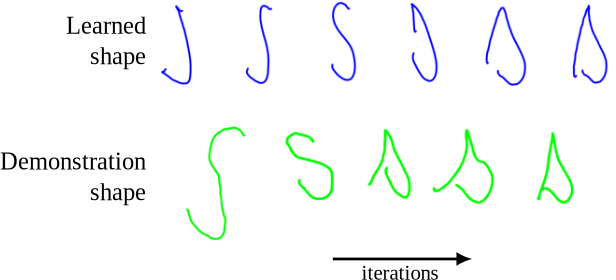
\includegraphics[width=0.6\columnwidth]{learningSdemo}
    \caption{\label{fig:demonstrationShapes2}Example of the learning algorithm
    responding (top) to user demonstration of shapes (bottom) for the letter `s'
    (demonstrations received from two 7-8 year-old children taking turns).}

\end{figure}


\subsubsection{Path Manipulation in the Letters' Eigenspace}

\begin{figure}[ht!]
    \centering
    \subfigure[Nine samples of the cursive ``h'', next to the reference]{
        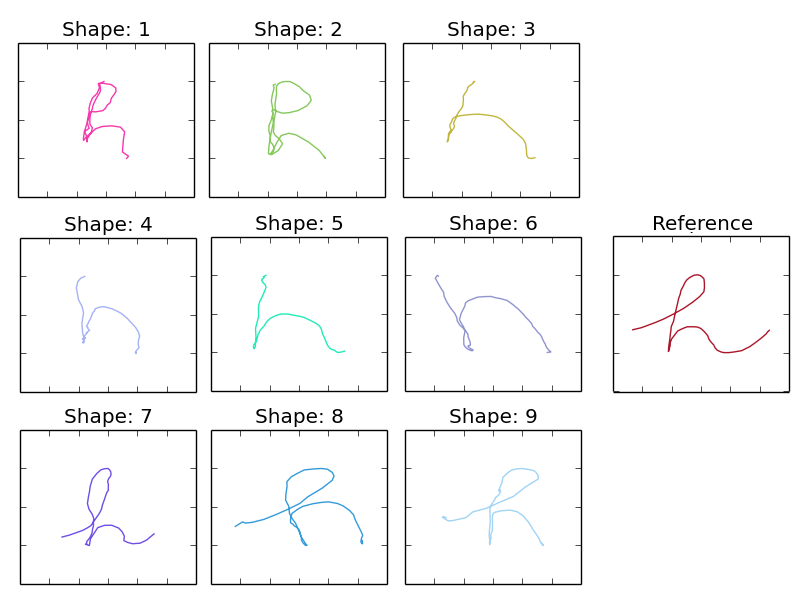
\includegraphics[height=6cm]{h}
    }
    \subfigure[Raw samples projected in the Eigenspace of the dataset]{
        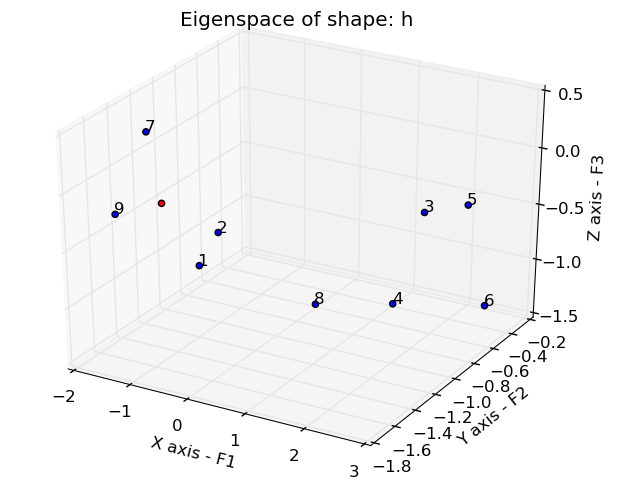
\includegraphics[height=4cm]{eigenspace-base}
    }
    \subfigure[Normalized samples, projected in the Eigenspace. The letters are
    clustered according to their styles.]{
        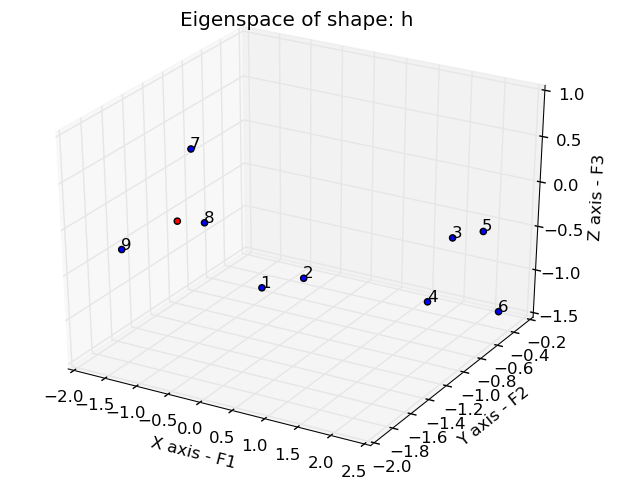
\includegraphics[height=4cm]{eigenspace-uniformization}
    }

    \caption{\small Projecting demonstrated letters onto the Eigenspace
    generated from the reference dataset effectively clusters the samples
according to their topological similarity.}
    \label{fig:stimuli}
\end{figure}


%%%%%%%%%%%%%%%%%%%%%%%%%%%%%%%%%%%%%%%%%%%%%%%%%%%%%%%%%%%%%%%%%%%%%%%%%%%%%%%%%%%
\subsection{Robotic Embodiement}
\begin{figure}[ht]
\centering

\resizebox{0.9\linewidth}{!}{%

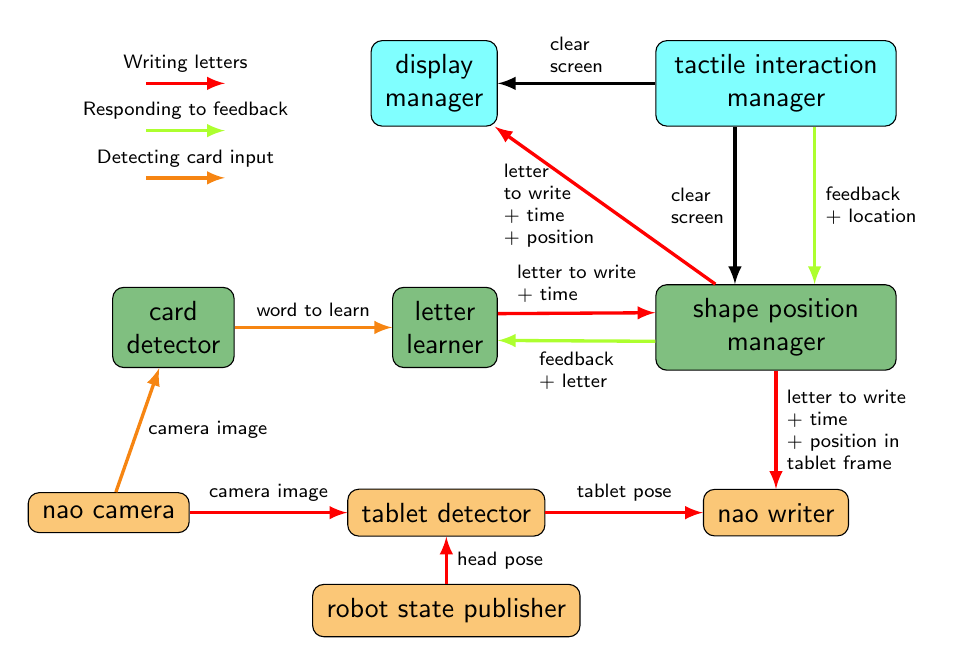
\begin{tikzpicture}[
    >=latex,
    node distance=2cm,
    every edge/.style={draw, very thick},
    redarrow/.style={fill=Red, draw=Red},
    greenarrow/.style={fill=GreenYellow, draw=GreenYellow},
    yellowarrow/.style={fill=BurntOrange, draw=BurntOrange},
    cmpt/.style={draw, align=center, rounded corners, inner sep=5pt, font=\sf, fill=black!20},
    label/.style={midway, align=left, font=\scriptsize\sf, fill=white, above,opacity=0,text opacity=1}]

    \node at (0,0)[cmpt, fill=Cyan!50, text width=2.7cm] (tactile) {tactile interaction \\ manager};
    \node[cmpt, fill=Cyan!50, left=of tactile] (display) {display \\ manager};
  
    \node [cmpt, fill=Green!50, below=of tactile, text width=2.7cm] (shape) {shape position \\ manager};
    \node [cmpt, fill=Green!50, left=of shape] (learner) {letter \\ learner};
    \node [cmpt, fill=Green!50, left=of learner] (card) {card \\ detector};

    \node [cmpt, fill=YellowOrange!50, below=1.5cm of shape] (writer) {nao writer};
    \node [cmpt, fill=YellowOrange!50, left=of writer] (tablet) {tablet detector};
    \node [cmpt, fill=YellowOrange!50, left=of tablet] (camera) {nao camera};
    \node [cmpt, fill=YellowOrange!50, below=0.6cm of tablet] (pose) {robot state publisher};

    %%% Relations between components
    \path (tactile) edge [->] node[label] {clear \\ screen} (display);

    \path ($(shape.north west)!0.33!(shape.north east)$) edge [<-] node[label,left] {clear \\ screen} ($(tactile.south west)!0.33!(tactile.south east)$);
    \path ($(shape.north west)!0.66!(shape.north east)$) edge [<-, greenarrow] node[label,right] {feedback \\ + location} ($(tactile.south west)!0.66!(tactile.south east)$);

    \path (shape) edge [->, redarrow] node[label, left, align=left] {letter \\to write \\ + time \\ + position} (display);
    \path (shape) edge [->,redarrow] node[label, right] {letter to write \\ + time \\ + position in\\tablet frame} (writer);

    \path ($(shape.north west)!0.66!(shape.south west)$) edge [->, greenarrow] node[label,below] {feedback \\ + letter} ($(learner.north east)!0.66!(learner.south east)$);
    \path ($(shape.north west)!0.33!(shape.south west)$) edge [<-, redarrow] node[label] {letter to write \\ + time} ($(learner.north east)!0.33!(learner.south east)$);

    \path (card) edge [->, yellowarrow] node[label] {word to learn} (learner);
    \path (camera) edge [->, yellowarrow] node[label, right] {camera image} (card);
    \path (camera) edge [->, redarrow] node[label] {camera image} (tablet);
    \path (tablet) edge [->, redarrow] node[label] {tablet pose} (writer);
    \path (pose) edge [->, redarrow] node[label, right] {head pose} (tablet);

    \path (-8, 0) edge [->, redarrow] node[label] {Writing letters} (-7, 0);
    \path (-8, -0.6) edge [->, greenarrow] node[label] {Responding to feedback} (-7, -0.6);
    \path (-8, -1.2) edge [->, yellowarrow] node[label] {Detecting card input} (-7, -1.2);
    
\end{tikzpicture}
}

\caption{Overview of the system. Components in the top row run on the tablet, 
those in the middle row on the central controller, and those in the bottom row 
on the robot.}

    \label{fig:archi}
\end{figure}



%%%%%%%%%%%%%%%%%%%%%%%%%%%%%%%%%%%%%%%%%%%%%%%%%%%%%%%%%%%%%%%%%%%%%%%%%%%%%%%%%%%
%%%%%%%%%%%%%%%%%%%%%%%%%%%%%%%%%%%%%%%%%%%%%%%%%%%%%%%%%%%%%%%%%%%%%%%%%%%%%%%%%%%
%%%%%%%%%%%%%%%%%%%%%%%%%%%%%%%%%%%%%%%%%%%%%%%%%%%%%%%%%%%%%%%%%%%%%%%%%%%%%%%%%%%
\section{Field Applications}

%%%%%%%%%%%%%%%%%%%%%%%%%%%%%%%%%%%%%%%%%%%%%%%%%%%%%%%%%%%%%%%%%%%%%%%%%%%%%%%%%%%
\section{Studies at School}

\begin{figure}
    \centering
    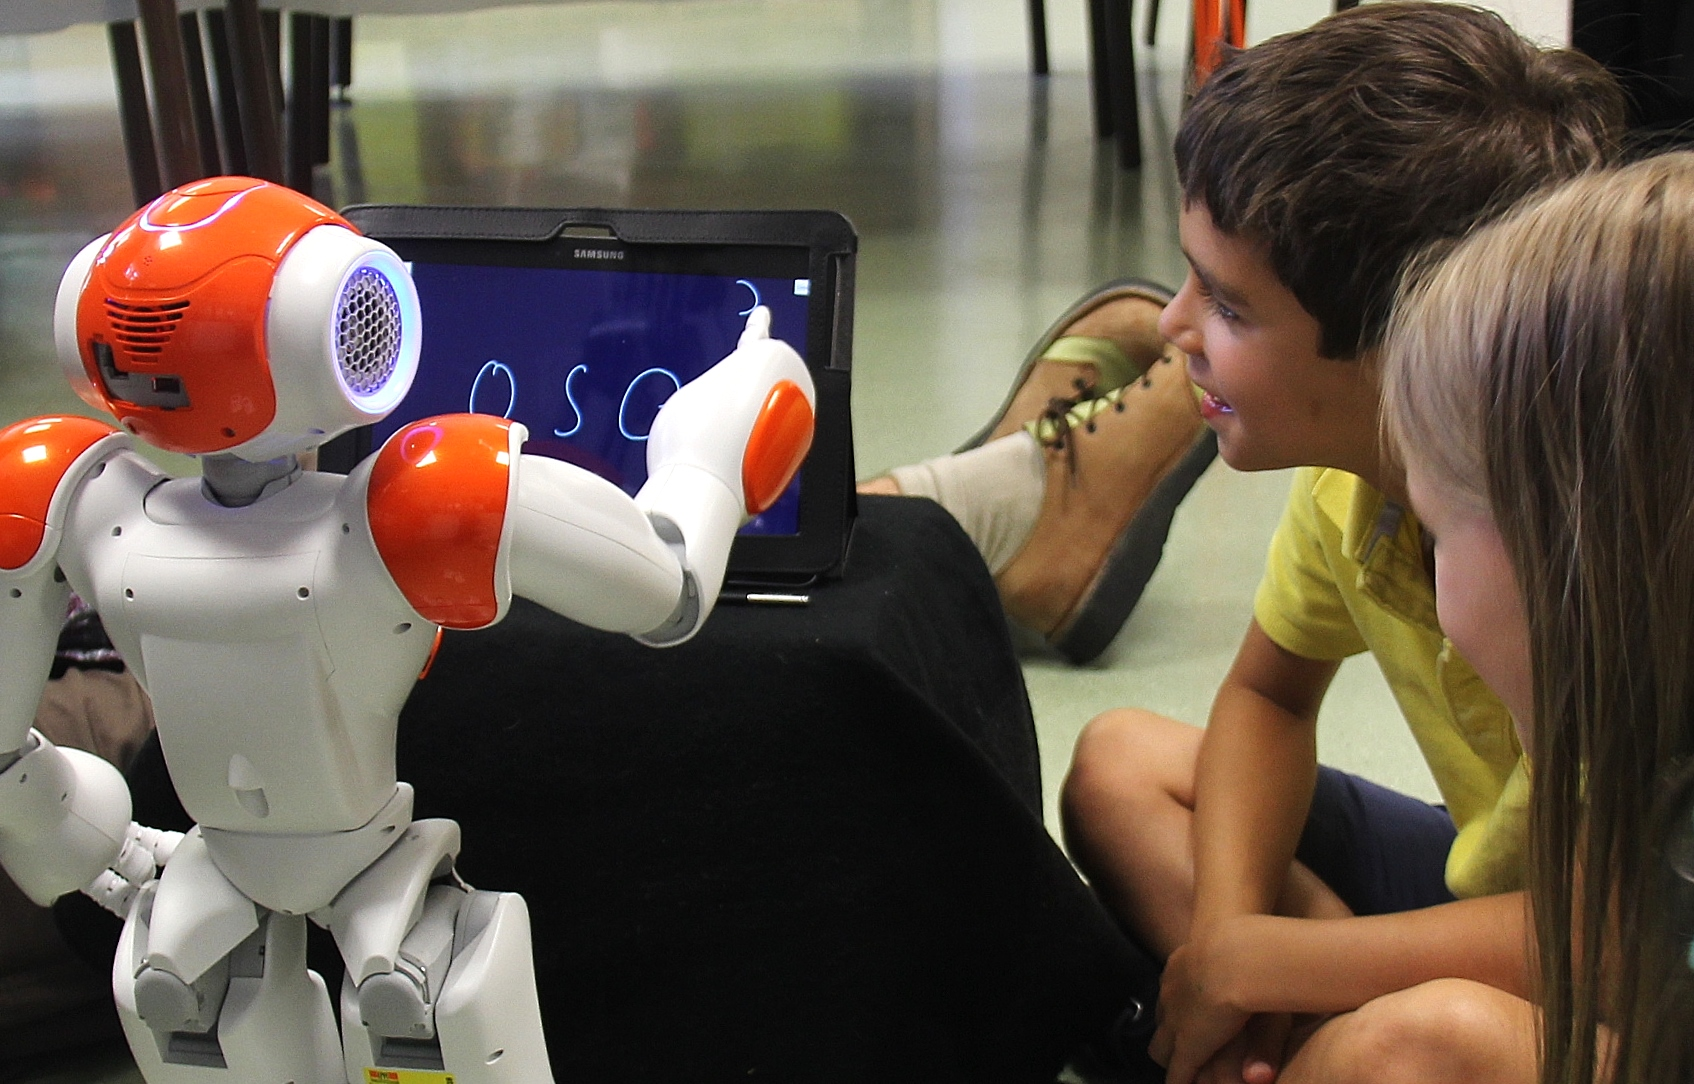
\includegraphics[height=3.9cm]{schools}
    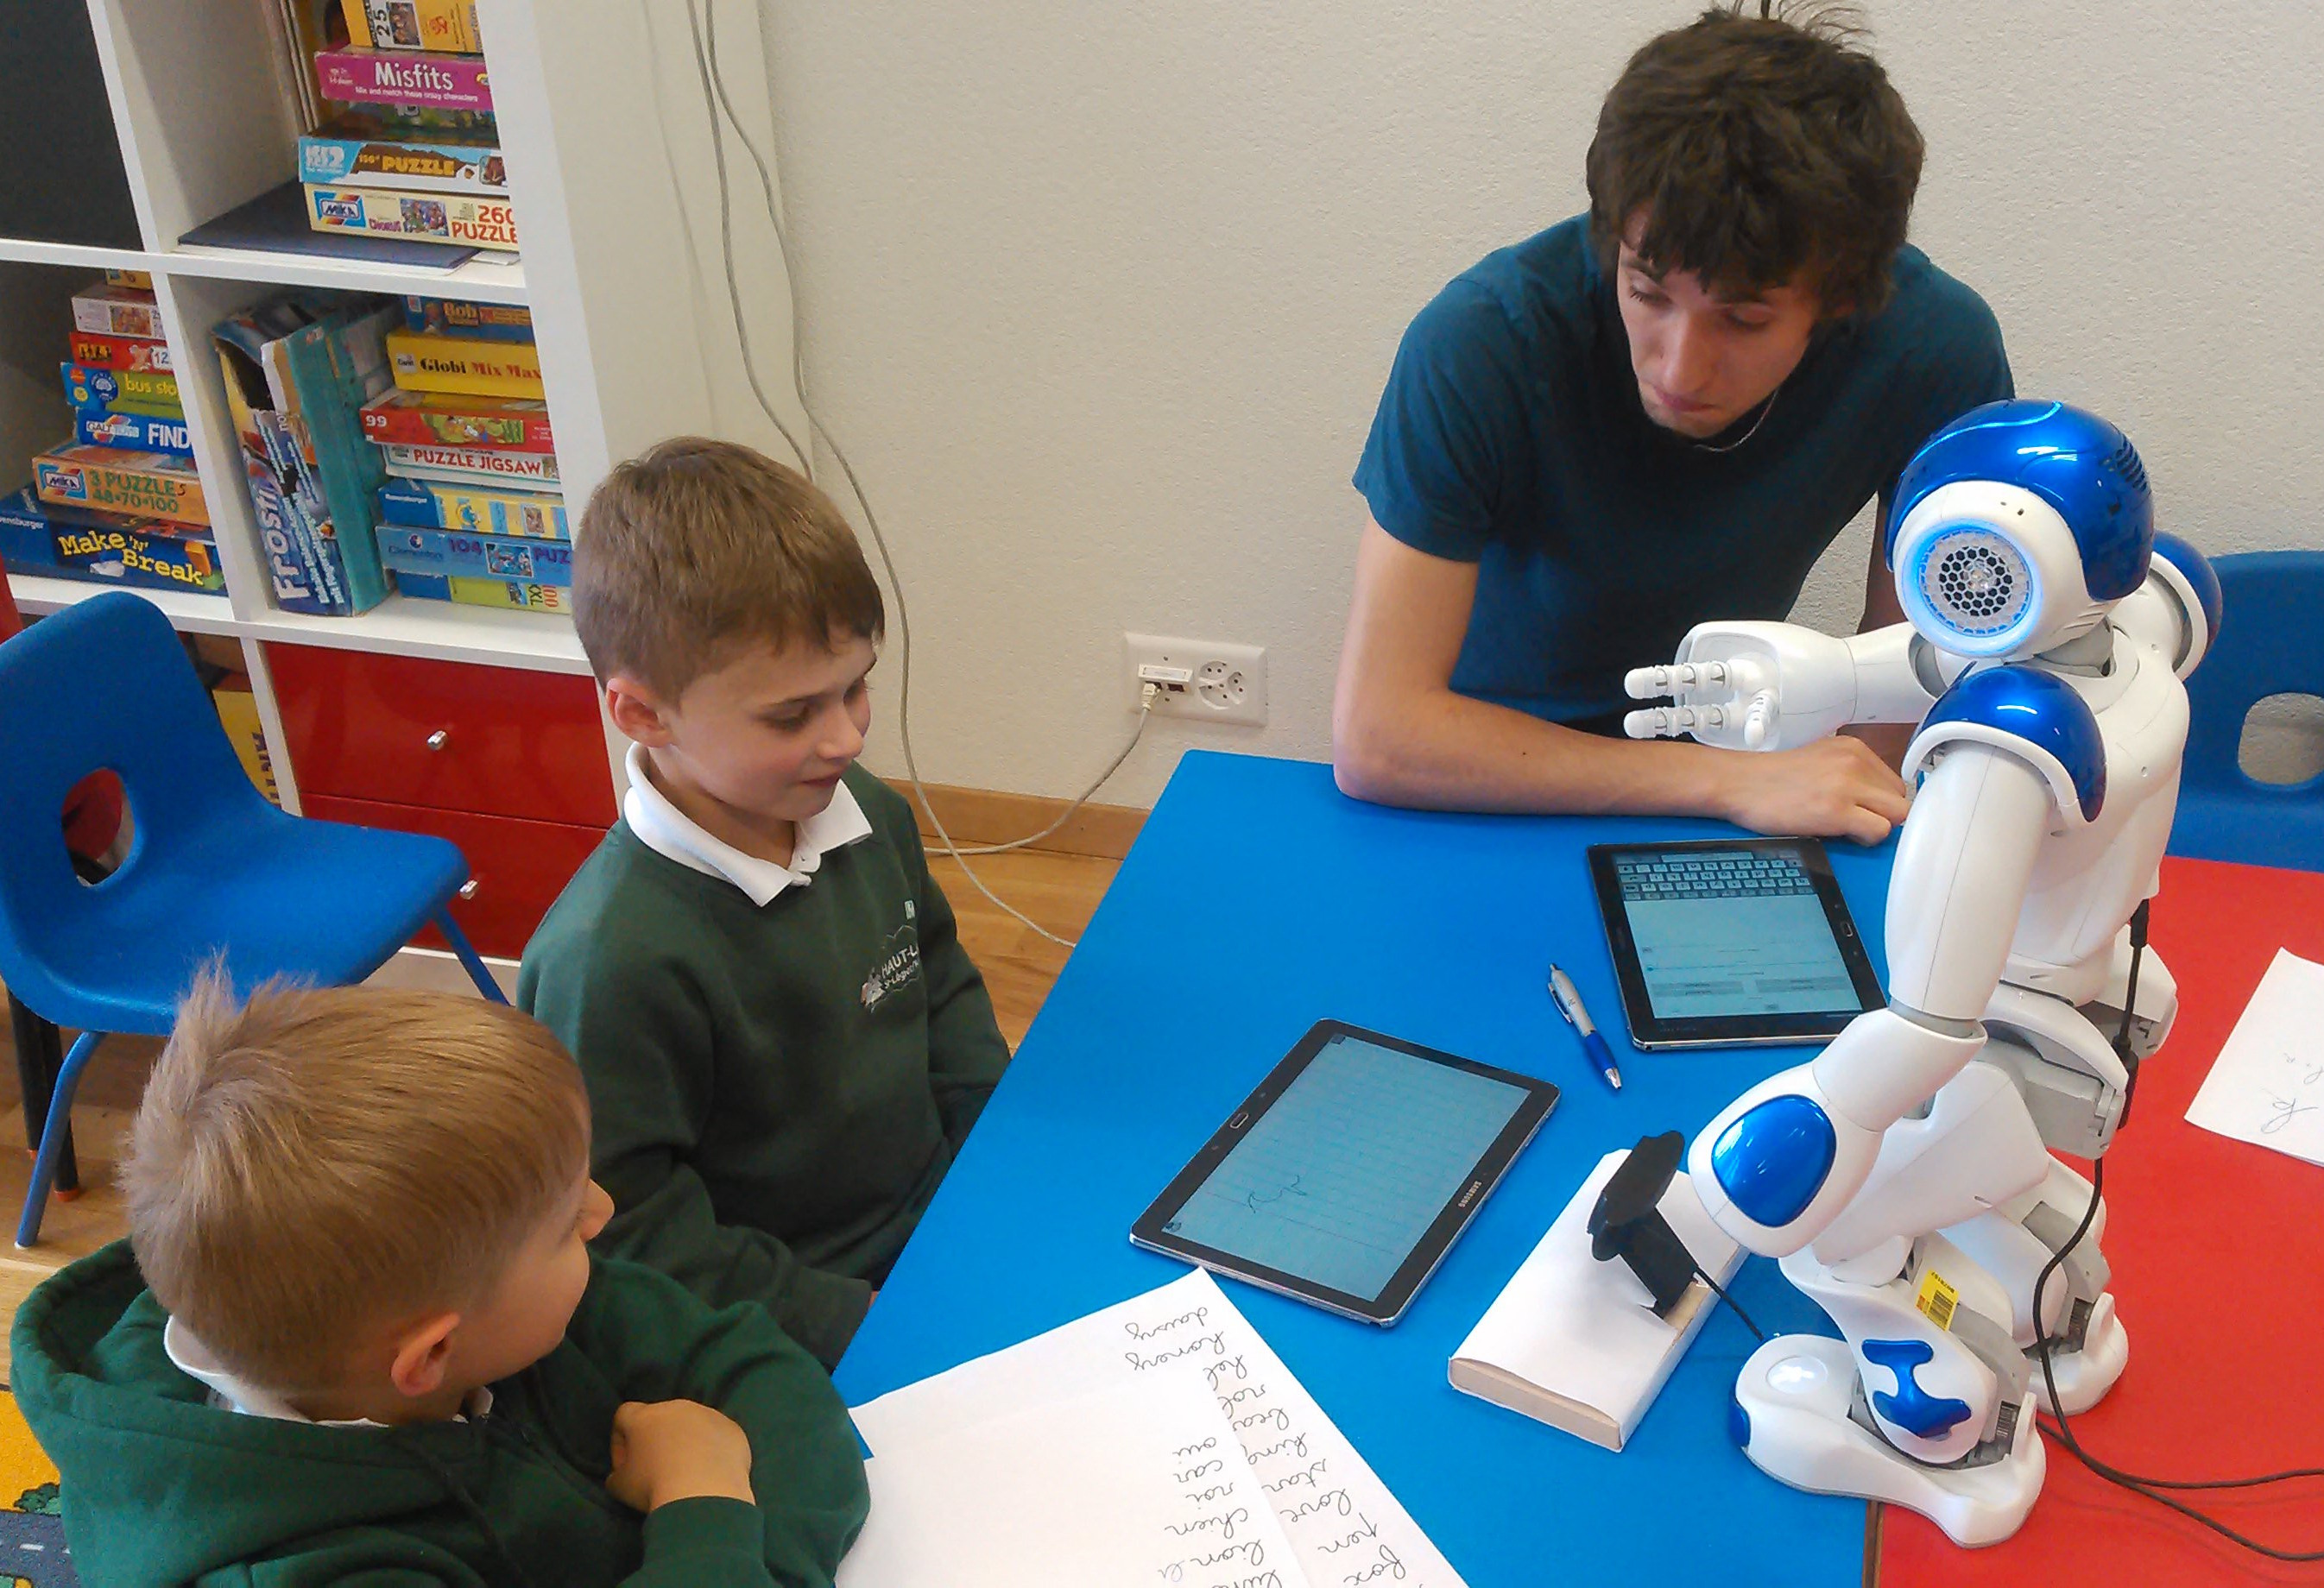
\includegraphics[height=3.9cm]{schools2}
    \caption{The first field studies were focused on technical validation, with
    above 100 pupils interacting with the robot over short periods (around 20
minutes), either alone or in small groups.}
    \label{fig:schools}
\end{figure}

%%%%%%%%%%%%%%%%%%%%%%%%%%%%%%%%%%%%%%%%%%%%%%%%%%%%%%%%%%%%%%%%%%%%%%%%%%%%%%%%%%%
\section{Case Study 1: Diego}

\subsection{Context, Study Design}

\begin{figure}
    \centering
    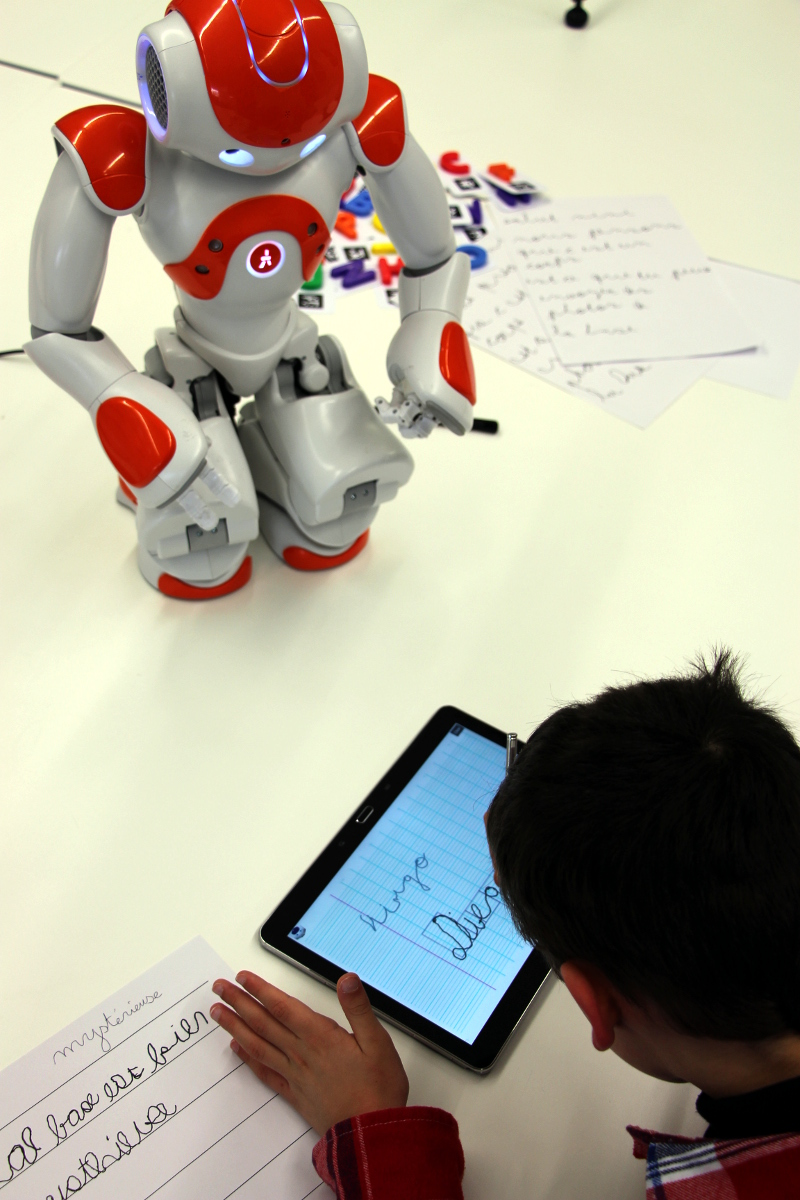
\includegraphics[width=0.5\linewidth]{diego}
    \caption{Diego working with Nao}
    \label{fig:diego}
\end{figure}


\subsubsection{Results}

\begin{figure}
    \centering
    \subfigure[Initial letter, generated by the robot]{
        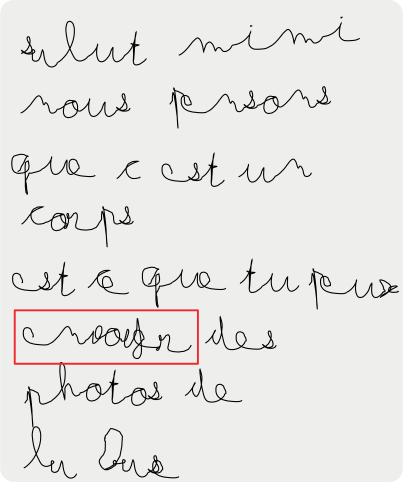
\includegraphics[height=6cm]{diego-initial-letter}
    }
    \subfigure[Final letter, after training with Diego]{
        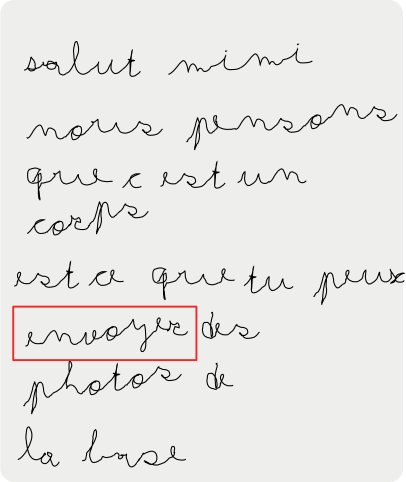
\includegraphics[height=6cm]{diego-final-letter}
    }

    \caption{\small Text generated by the robot, before and after training with
    the child. As an example, the red box emphasizes the changes on the word
    ``envoyer''.}
    \label{fig:stimuli}
\end{figure}


%%%%%%%%%%%%%%%%%%%%%%%%%%%%%%%%%%%%%%%%%%%%%%%%%%%%%%%%%%%%%%%%%%%%%%%%%%%%%%%%%%%
\subsection{Case Study 2: Henry}

\subsubsection{Context, Study Design}

\begin{figure}
    \centering
    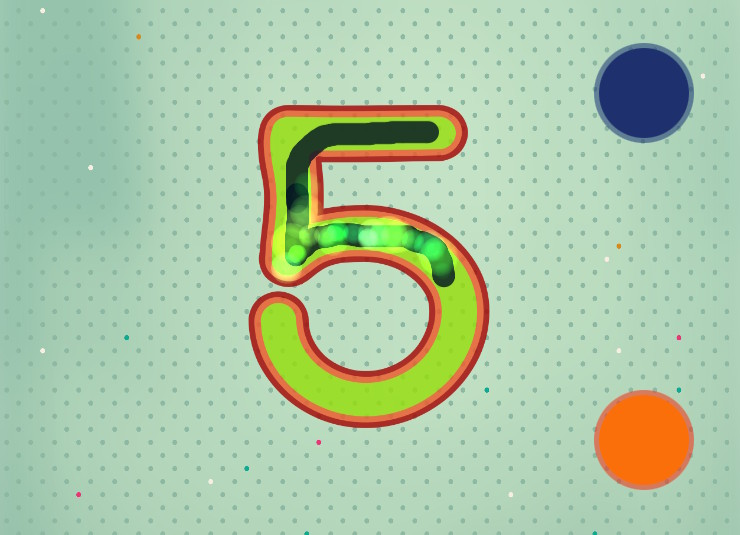
\includegraphics[width=0.9\linewidth]{abc-writer}
    \caption{Screenshot of the Android application developed to be used as
    pre-test and post-test: the child must follow with his finger the path of
the letter or number. We count the number of times the finger goes outside of
the red-bordered area.}
    \label{}
\end{figure}


\subsubsection{Results}

\begin{figure}
    \centering
    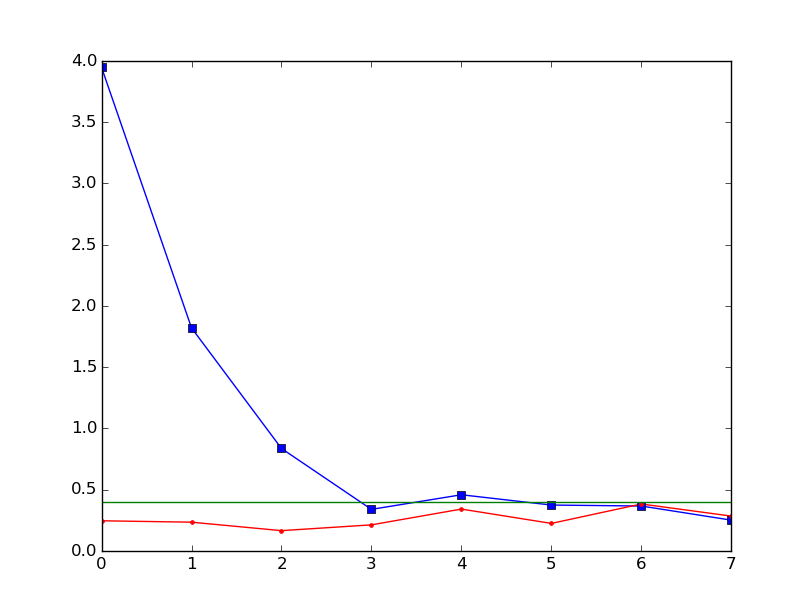
\includegraphics[width=0.9\linewidth]{learning_6}
    \caption{Progresses made by Henry over one 45-minutes interaction session
    while writing ``6''.}
    \label{}
\end{figure}



%%%%%%%%%%%%%%%%%%%%%%%%%%%%%%%%%%%%%%%%%%%%%%%%%%%%%%%%%%%%%%%%%%%%%%%%%%%%%%%%%%%
%%%%%%%%%%%%%%%%%%%%%%%%%%%%%%%%%%%%%%%%%%%%%%%%%%%%%%%%%%%%%%%%%%%%%%%%%%%%%%%%%%%
%%%%%%%%%%%%%%%%%%%%%%%%%%%%%%%%%%%%%%%%%%%%%%%%%%%%%%%%%%%%%%%%%%%%%%%%%%%%%%%%%%%
\section{Agency and Commitment}

However, we believe that the strongest impact of this work is for the
human-robot interaction community and relates to the very \emph{nature} of the
interaction fostered by this research. The work presented here investigates a
particular role for a robot in the education of handwriting: not only is the
robot actively performing the activity by drawing letters, but it does so in a
way that engages the child in a very specific social role. The child is the
teacher in this relationship and the robot is the learner: the child must engage
in a (meta-) cognitive relationship with the robot to try to understand why the
robot fails and how to help it best.  Here, the robot is more than just an
activity facilitator or orchestrator -- its physical presence and embodiment
induce agency and anthropomorphising, and cognitively engage the child into the
learning activity, which we predict will lead to higher learning efficacy.


%%%%%%%%%%%%%%%%%%%%%%%%%%%%%%%%%%%%%%%%%%%%%%%%%%%%%%%%%%%%%%%%%%%%%%%%%%%%%%%%%%%
%%%%%%%%%%%%%%%%%%%%%%%%%%%%%%%%%%%%%%%%%%%%%%%%%%%%%%%%%%%%%%%%%%%%%%%%%%%%%%%%%%%
\section*{Acknowledgments}

We would like to thank Deanna Hood for her key contribution to the project.
This research was partially supported by the Funda\c{c}\~{a}o para a Ci\^{e}ncia
e a Tecnologia (FCT) with reference UID/CEC/50021/2013, and by the Swiss
National Science Foundation through the National Centre of Competence in
Research Robotics.

\bibliographystyle{abbrv}
\bibliography{biblio}


\end{document}
